%___________________________________________________________________________________________________
\chapter{Operations with functions}     \label{chap:opfuncs}

    \section{Introduction} 

One of the paradigms grouped within the declarative programming is the functional programming paradigm,
which finds its bases in mathematics and more specifically in lambda calculus.
With this paradigm every piece of code uses pure mathematical style and is built 
under two main ideas: the functions are only applied to arguments 
and the functions are combined to create new functions. 

Some programming Languages that support functional programming are 
Haskell, JavaScript, Lisp, Erlang or Scala.
Although Fortran and Python are not functional programming languages, they
take several principles and ideas from this paradigm such as pure functions or first-class/higher-order functions,
the latter, introduced below, is intensively used in this chapter. 

%f matematica vs f lambda
In mathematics a function is a relation 
from elements of a set $X$ of inputs (domain) 
to elements of a set $Y$ of outputs (codomain) 
where each input is related to exactly one output.
$$ 
\myfunc{ f }{X}{Y}{x}{f(x) = x^2} 
$$
\newpage
A function in a language like Fortran follows the same concept:
\begin{verbatim}
function f(x) 
    real, intent(in) :: x
    real :: f

    f = x**2
    
end function
\end{verbatim} 
Notice that, in lambda calculus and functional languages, functions are much the same but anonymous, 
which means they do not have an identifier associated to denote them. 

This chapter covers the equivalent of some mathematical analysis tools translated to scientific programming. 
Piecewise-defined functions, plotting of functions, integrals and derivatives or series expansions of functions 
are some of the first things that a scientific programmer should know to solve problems. 
All these tools, when expressed in a program, can make intensive use of higher-order functions: 
those functions that can take one or more functions as arguments 
or can return a function as a result.

The examples presented here are developed with Fortran and Python, however, the concepts are cross languages. 
For example, the ideas around the approximation of a derivative or integral with a computer or 
the consequences of using finite precision to represent real numbers
are similar in any language. 

 
%Its properties are covered later in the Advance Programming chapter. 
%Try now to glimpse with these examples some of its advantages comparing it to the imperative programming.
%It seeks to have each line of code made up of mathematics which, 
%although it only needs from variables and functions to work, is extremely powerful.

%Modularity is a key property in a well-structured software, it simplifies debugging, allows to test independent pieces of code and code reuse.  
%Hence, considering the basic principles of the paradigm and the qualities inherited from being a declarative paradigm,
%functional programming has the potential to make a program 
%short, effective, easy and part by part debuggable, reusable, maintainable, testable, predictable, and well-structured among others. 

    %___________________________________________________________________________________________________
    \newpage
    \section{Defining piece-wise functions} \label{sec:piecewise}

A function can be defined by means of one or more formulas, a list of values, a recurrence rule, etc. 
In this example, the following piece-wise mathematical function is defined in Fortran 
using three formulas for different intervals of its domain:

$$ 
\myfunc{ f }{\mathbb{R}}{\mathbb{R}}{x}{f(x)} 
$$

$$
f\left( x\right) = 
\begin{cases}
     0,  \ \ \ \  \ \ \ \ \  x < -\frac{\pi}{2}       \\
     \cos(x), \ \             x \in\left[ -\frac{\pi}{2}, \frac{\pi}{2}   \right)        \\ 
     0, \ \ \ \  \ \ \ \ \   x \geq \frac{\pi}{2}
\end{cases}
\label{eq:piecewise}
$$

It can be easily done through a conditional expression on the variable $ x $ so, for each point of the domain the proper result is returned. 
From the numerical point of view two precautions must be taken into account:

\begin{itemize}
    \item In the first place, make sure that the entire domain of the function 
    is represented in the code, do not forget to consider all the intervals. 
    It is possible that the domain of the function is not the whole set $\left\{ \mathbb{R} \right\} $, 
    however, the function in the code may be called with values $ x $ out of the domain. 
    A big topic is opened under this premise; how can be the output of an out-of-domain value managed.
    
    \item In the second place, for the algorithm the order in which we define the 
    intervals is important. Consider what function we would be representing if the 
    conditional \texttt{( x < PI/2 )} is written in the first place
    and the conditional \texttt{( x < -PI/2 )} in the second place for this same example.
    
\end{itemize}


\newpage
%\vspace{0.5cm} 
\renewcommand{\home}{./Fortran/sources/Foundations/Calculus}
\listings{\home/Examples/Integrals_derivatives.f90}{function Piecewise_f}
{end function}{Integrals_derivatives.f90}

\vspace{-0.7cm} 
\subsection*{Python code} 
The same code written with Python is more straight-forward,
this function definition with an \texttt{if/else} structure is a good example. 
Remember that implicit typing can make programming simpler but can also lead to unpredictable results or errors difficult to debug.
\vspace{0.3cm}
\renewcommand{\home}{./Python/sources/Foundations/Calculus} 
\lstpython
\listingsp{\home/Examples/Integrals_derivatives.py}{def Piecewise_f}
{x > pi}{Integrals_derivatives.py}
\lstfor


    %___________________________________________________________________________________________________
    \vspace{-0.5cm}
    \section{Plotting functions}

For a mathematical function its graph is one of the ways to represent it. 
Notice that for a given function $ f(x) $ the set of all pairs 
$ \left\{ ( x, f(x) ) \mid x\in D \right\}$ (where $D$ is the domain of the function) 
are unique.

This is specially useful when the domain and codomain of the function are subsets of $\mathbb{R}$
or maybe the domain is a subset of $\mathbb{R}^2$ since the elements $(x,y)$ or $((x,y),z)$ can be 
associated to points in a coordinate system resulting in a curve in 2 dimensions or a surface in 3 dimensions. 
The graph of functions, results, variables, etc. is used for ``graphic debugging'', an essential way to debug 
scientific programs like simulations in physics. 
It makes much easier to find all kind of bugs in a program 
by means of plotting final or intermediate results obtained by the computer.  

The following example is based on DISLIN, a plotting library for Fortran and C languages created by the
Max Planck Institute. It is a high-level plotting library for displaying
data that can be called from the main program or subroutines.

\vspace{0.5cm}
\renewcommand{\home}{./Fortran/sources/Foundations/graphs} 
\listings{\home/plotting.f90}{subroutine plot}
{end subroutine}{plotting.f90}
\renewcommand{\home}{./Fortran/sources/Foundations/Calculus} 

\vspace{-.5cm}
The previous subroutine allows to plot a 201 points curve from a generic function declared (by means of an interface) as a:
$$ 
\myfunc{ \texttt{f\_R\_R} }{\mathbb{R}}{\mathbb{R}}{x}{\texttt{f\_R\_R(x)}} 
$$

It is used in combination with an initialization subroutine for the graph and a subroutine that displays the result (the Fortran solution that accompanies this book shows some examples of how to use this subroutines and DISLIN libraries):

\texttt{subroutine plot\_ini( xmin\_, xmax\_,  ymin\_, ymax\_ )} 

\texttt{subroutine plot\_show(  )}

Notice how this subroutine makes use of the \texttt{parameter M} that needs to be converted to \texttt{real} when the grid \texttt{x} is calculated to avoid operating in the integer field. Also, the use of implicit loops greatly simplifies the reading of the code.






    %___________________________________________________________________________________________________
    \newpage 
    \section{Integrals and derivatives of functions}   \label{sec:intder}

Let's build a simple approximation to the derivative of a function $ f(x) $ by means of its definition:

$$
f'(x) = \lim_{h\rightarrow 0}\frac{f(x+h)-f(x)}{h}
$$

In calculus, the existence of this limit (derivable function) implies that both lateral limits exist, are finite and equal (at least when the function is defined in both sides of the point $x$):

$$
    f'(x) = \lim_{h\rightarrow 0^-}\frac{f(x+h)-f(x)}{h} = \lim_{h\rightarrow 0^+}\frac{f(x+h)-f(x)}{h}
$$

To obtain an approximation to this value $ f'(x) $ in a point $x $ with the computer, finite differences can be used. Instead of reproducing the limit in the point, a fixed value of $ h \neq 0$ is used. Notice that both $ h > 0 $ or $ h < 0 $ are possible so the approximation can be found like a forward difference or a backward difference. Actually, also central differences can be used if the expression is slightly modified. What must be considered is that now each expression leads to a different approximation while in calculus the existence of the derivative implies that all values are equal. 

For this case let's consider $ h > 0 $ with $h$ a small value:

$$
    f'(x) \simeq \frac{f(x+h)-f(x)}{h}
$$

The question that arises; is it possible to bound the error of the approximation? 

$$
    E = f'(x) - \frac{f(x+h)-f(x)}{h}
$$

If the function $f(x)$ is sufficiently smooth near $x$ (for a forward-difference twice differentiable is needed), then a Taylor expansion can be used so the order of the scheme used is obtained. Intuitively, it is clear that by lowering the value of $h$ a better approximation of the derivative is obtained. Finding the order of the scheme means precisely finding how fast the error tends to zero when $h\rightarrow 0$. In addition, round-off error appears in this approximation depending on the value of $h$ too.

Let's bound the truncation error for a forward difference. Starting with the Taylor series of $f(x)$ at the point $x$ particularized in $x+h$:

$$
f(x+h) = f(x) + h f'(x) + \frac{h^2}{2} f''(x) + \mathcal{O}(h^3) 
$$

Notice that $\O(h^3)$ means that the following terms are lower than a constant times $h^3$. Re-arranging the expression:

$$
\frac{f(x+h) - f(x)}{h} = f'(x) + \frac{h^2}{2h} f''(x) + \mathcal{O}(h^2) = f'(x) + \frac{h}{2} f''(x) + \mathcal{O}(h^2) 
$$

$$
\abs{\frac{f(x+h) - f(x)}{h} - f'(x)}  \  \leq  \    C h  
$$

The error committed by replacing the derivative $f'(x)$ by the finite difference approximation is of order $h$ and the same result is obtained if backward-difference is used. Of course this is not the only way to approximate the value of a derivative. First of all, central differences could be used and, if the function is three times differentiable the truncation error of that approximation can be demonstrated that is of order $h^2$. Secondly, higher order finite differences exist so the value of a first derivative can be approximate with order $h^4$, $h^6$, etc. considering more points of the domain, while the example shown here comes from the derivative definition or the Taylor series expansion similarly, higher order approximations can be inferred from the interpolation theory. Thirdly, other strategies that also comes from the interpolation theory can be used so spectral convergence can be obtained (see section \ref{sec:convergence}). 

A different source of discrepancy between the real value and the approximation appears; round-off error, also dependent on the value of $h$ taken. Notice that as $h$ gets smaller, the values of $f(x+h)$ and $f(x)$ become more similar. This issue, with infinite precision arithmetic would not pose any problem, however, performing the subtraction with the computer's finite precision involves the problem of numerical cancellation. This topic is broaden in the chapter \ref{sec:cancellation} since the basis of real numbers representation are explained. For now, just keep in mind the following:

\begin{itemize}
    \item Every real numbers in the computer is stored with a rounded value that fits in the finite precision used by the computer. Consider for example the numbers $1.2345651$ and $1.2345649$, in a finite precision machine they could be stored only with 6 significant digits and they would become: $1.23457$ and $1.23456$, they have been rounded. Of course, both values $f(x+h)$ and $f(x)$ in our derivative computation suffer from this issue.
    
    \item When two near values are subtracted the significant digits are reduced, i.e. from 6 significant digits in the following expression we end up with just 1: 
    
    $$
    1.23457 - 1.23456 = 0.00001 = 1\cdot 10^{-5}
    $$
    
    \item If both values are approximated to the sixth digit and the result of the subtraction is a value in the order of magnitude imposed by that digit, then it is dominated by the round off made to the numbers!
     In this example the infinite precision operation would result in $1.2345651 - 1.2345649 = 2\cdot 10^{-7}$ quite smaller than the result obtained by the finite precision machine. 
\end{itemize}

Our expression for the derivative $\frac{f(x+h)-f(x)}{h}$ will have an error in the numerator divided by $h$ so, with no deeper explanations let's say now that this rounding error can be bounded by the following expression. Notice how it depends inversely on $h$ so it is a barrier for the reduction of h as a way to increase the accuracy of the derivative. The decision and meaning of writing $2\epsilon$ for the numerator error is deeply treated in the chapter \label{chap:reals}.  

$$
E_{round} = \frac{2\epsilon}{h}
$$

Since we could be interested in making $h$ as small as possible to obtain better approximations to the derivative, it is not difficult to find that round-off barrier in our computations. Both sources of error can be dominant and it is essential to understand the origin of both and how to relate the precision desired for a simulation (needs of the project) and the way to approximate derivatives with the computer. 

%------------------------------------------------------------------------------------------
The following codes recycles the procedure interface used along this chapter of \texttt{f\_R\_R(x)} for the function \texttt{f} and defines the \texttt{Derivative} function with inputs the function to derive and the value where obtaining the approximation. Notice that this new function itself also responds to the interface:

$$ 
\myfunc{ \texttt{f\_R\_R} }{\mathbb{R}}{\mathbb{R}}{x}{\texttt{f\_R\_R(x)}} 
$$

\newpage
\vspace{0.5cm}
\listings{\home/Calculus.f90}{Derivative}
{end function}{Calculus.f90}

\vspace{0.5cm}
\listings{\home/Calculus.f90}{interface}
{end interface}{Calculus.f90}


%------------------------------------------------------------------------------------------

Now let's compute the definite integral of a function $f(x)$ in the closed interval $ [a,b] $ and let's do it in a functional way as it is common during this book.
In this case we are going to obtain an approximation to the integral value through a Riemann sum, which means that the area of the curve under the function in the interval is obtained as a sum of small rectangles along the interval and carrying that process to the limit. 

$$ 
\int_{a}^{b}f(x)dx   =   \lim_{m\rightarrow \infty}\sum_{i=0}^{m-1}f(x_i) \Delta x
$$

Each value $x_i$ is taken from a partition of $[a,b]$:

$$
x_i = a + i\Delta x \ \ \    \text{with} \ \ \  i = 0, ..., m-1
$$ 

and with:

$$
\Delta x = \frac{\mid b-a\mid}{m}
$$

However, we need an approximation so instead of evaluating that limit, we choose a value $m$ big enough to accomplish with the accuracy required. 

$$ 
\int_{a}^{b}f(x)dx   \simeq \sum_{i=0}^{m-1}f(x_i) \Delta x
$$

In this example, the leftmost value of each subinterval is taken to approximate the rectangle area, however, the rightmost value or another point contained in the interval could be used. 

%------------------------------------------------------------------------------------------

\vspace{0.5cm}
\listings{\home/Calculus.f90}{Integral}
{end function}{Calculus.f90}

Some notes should be taken from this example: firstly, notice that the initial value given to \texttt{dx} is not the actual value used, it is just an approximation to the expected value  (\texttt{0.001}). The operation \texttt{abs(b-a)/dx} is used to calculate the approximate number of subintervals that fit in our interval $[a,b]$ and then the integer part is retained. Then, the exact value of  \texttt{dx} is calculated for an integer number of subintervals. Secondly, notice that the sum must not stop in the last value of the interval ($b$) but in the previous one since the area of that rectangle is computed by $dx\cdot f(a+dx(m-1))$. As usual, the whole addition can be compacted in the sum of the components of a vector defined by an implicit loop. 


\newpage 
\subsection*{Python code} 
Find the same example coded with Python, there is no need of explicitly declare an interface between the argument function \texttt{f} and the functions \texttt{Derivative( f, x )} and \texttt{Integral( f, x )}. 
\renewcommand{\home}{./Python/sources/Foundations/Calculus}

\vspace{0.5cm}
\lstpython
\listingsp{\home/Calculus.py}{def Derivative}
{return}{Calculus.py}
\lstfor

\vspace{0.5cm}
\lstpython
\listingsp{\home/Calculus.py}{def Integral}
{return}{Calculus.py}
\lstfor

 



    %___________________________________________________________________________________________________
    \newpage 
    \section{Examples of operations with functions}

The following subroutine gives some examples of the functions seen during this chapter. 
DISLIN is used for all the graphs as mentioned before. Firstly, the plot intervals must 
be initialize so the \texttt{plot\_ini} subroutine is used and the plotting boundaries 
are declared, all the graphs will be calculated and represented in 
$x\in \left[ -2\pi, 2\pi \right]$, 
$y\in \left[ -2.5, 2.5 \right]$.
Then, four functions are represented; a sine, 
the piecewise function defined in \ref{eq:piecewise},
its derivative and 
its integral from $-1$ to x. 

To graph those functions with \texttt{plot( f )}, the single input argument needed is the function itself.  
Also, the already explained \texttt{procedure (f\_R\_R) :: f} is used for \texttt{f}. Hence,
the functions \texttt{Derivative\_f(x)} and \texttt{Integral\_f(x)} are needed to 
build the following mathematical expressions: 

$$
\text{\texttt{Derivative\_f}}(x) = \frac{df(x)}{dx}
$$

and:

$$
\text{\texttt{Integral\_f}}(x) = \int_{-1}^{x} f(x) dx
$$

Remember that $f(x) = \text{\texttt{Piecewise\_f(x)}}$. Notice that integrating the function with these limits implies finding one of the primitive functions of $f(x)$, that one where the not defined constant has a specific value decided by the lower integration limit $x=-1$. The function treated in this example is positive (or zero) in the whole domain of definition so its integral as well. However, since it is plotted starting in $x = -2\pi$ and the function is integrated from $x=-1$, we expect the result to be negative until it reaches zero in $x=-1$ according to this property of definite integrals:

$$
\int_{-1}^{x} f(x) dx = - \int_{x}^{-1} f(x) dx
$$

\newpage 
\vspace{0.5cm}
\renewcommand{\home}{./Fortran/sources/Foundations/Calculus}
\listings{\home/Examples/Integrals_derivatives.f90}{Integral_and_derivative_examples}
{end subroutine}{Integrals_derivatives.f90}
 
 \newpage 
 \subsection*{Python code} 
 \renewcommand{\home}{./Python/sources/Foundations/Calculus}
 \lstpython
 \listingsp{\home/Examples/Integrals_derivatives.py}{def Integral_and_derivative_examples}
 {end}{Integrals_derivatives.py}
 \lstfor
 

    %___________________________________________________________________________________________________
    \section{Series expansion} 

One of the main focus of numerical methods is to approximate functions by means of different expansions: 

\begin{enumerate} 
\setlength\itemsep{-0.1cm}
	\item Polynomial expansion: Taylor, Lagrange.
	\item Trigonometric series: sine and cosine expansions. 
	\item Expansion by means of known basis: Chebyshev, Legendre, etc. 
\end{enumerate} 

The same function can be expanded or approximated with different basis.
It goes without saying that the computer only allows to sum a finite number $ N $  of terms. 

Hence, the best election is related to the rate of convergence 
of the expansion. In other words, given a tolerance error between the approximation and the exact function, 
the best expansion allows to obtain the approximation with a minimum number of terms $N$. 



        %___________________________________________________________________________________________________
        \newpage
        \subsection{Taylor expansions of functions} 
   
One of the most used series expansion of a function is its Taylor series, without going any further, in section \ref{sec:intder} we have used 
a Taylor expansion to estimate the truncation error committed when approximating the derivative of a function by its finite difference 
expression.

In general, as already mentioned, a series expansion is a very useful way to approximate the value of a given function in a domain. More 
specifically, the Taylor series, which uses power series, allows us to estimate the value of a function at one point from its value and the 
value of its derivatives at a different point. Polynomials are extensively known and they are easy to derive, integrate, multiply, etc. so 
treating a function as its power series approximation can have many advantages when it comes to operating with that function.

A power series of the function $f(x)$ (centered in $x_0 = 0$ and with $N+1$ terms) can be expressed as:
%\[  f(x) = \sum_{k=0} ^N a_k \  x^k, \qquad \qquad a_k = \frac{  f^{(k)} (0)  }{ k! },  \]  
 
\[  f(x) \approx \sum_{k=0} ^N a_k \  x^k,  \] 

where $a_k$ are real numbers that depend only on $k\in \mathbb{N}$ and not on $x$. These coefficients are calculated as:

$$
a_k = \frac{  f^{(k)} (0)  }{ k! }  
$$

being $f^{(k)} (0)$ the \textit{k}-th derivative of $f(x)$ in the point $x_0 = 0$.
 
For a Taylor expansion around a generic point $x_0$ the shape of the polynomial series and the coefficient expressions are:

\[  f(x) \sim \sum_{k=0} ^N a_k \  (x - x_0)^k, \qquad a_k = \frac{  f^{(k)} (x_0)  }{ k! }   \] 





Let's take a look at the Taylor expansion functions proposed here (written with a declarative style). Two approximations are used, one is 
called under the expected minimum value to be added to the series (epsilon), the other is directly called with the number of terms to be 
added. Imitating a multilayer structure, previous functions can be recycled, for example \texttt{TaylorE} needs to sum as many terms as the 
epsilon value requires so the function \texttt{Sigma} function (seen in chapter \ref{sec:Sigma}) is used. In a different way, 
\texttt{TaylorN} is directly based on \texttt{Sigma\_N} since the number of terms to be added are known and declared as an argument.

Despite that, the structure of both functions is the same, a declaration of the Taylor expansion definition. The \texttt{Sigma} function is 
called with the general term of the series, the first term to add (which is 0 in this kind of power expansion) and the condition to stop 
(epsilon value or number of terms). Those are the only ingredients needed to compute the sum series that returns the value of the Taylor 
expansion in a point $x$. 
  
\vspace{0.5cm}
\renewcommand{\home}{./Fortran/sources/Foundations/Calculus} 
\listings{\home/Taylor_expansions.f90}{function TaylorE}
   {end function}{Taylor_expansions.f90}
   
\renewcommand{\home}{./Fortran/sources/Foundations/Calculus}       
\listings{\home/Taylor_expansions.f90}{function TaylorN}
   {end function}{Taylor_expansions.f90}
   

\newpage   
A couple of details should be noticed here. First of all, the derivatives of the function to be expanded are introduced as an argument in 
\texttt{Taylor} function. The arguments of this function must be the value where deriving and its order. To do that, a generic procedure is 
used so it can be recycled next time a function of the same form is used:

$$ 
\myfunc{ \texttt{f\_RxN\_R} }{\mathbb{R} \times\mathbb{Z}}{\mathbb{R}}{\left( x,k \right)}{\texttt{f\_N\_R(x,k)}} 
$$
   
Secondly, both functions are overloaded into one called \texttt{Taylor} so the particularities of each one are transparent for the user, just 
call a generic function specifying an epsilon value or a number of terms as fourth argument, the calculation is correctly performed 
automatically. Notice that the \texttt{type} of argument must always be respected so \texttt{N}, the number of terms, must be an 
\texttt{integer} value and \texttt{eps}, on the contrary, must be a \texttt{real} value.  
   
    
\vspace{0.5cm}   
\renewcommand{\home}{./Fortran/sources/Foundations/Calculus} 
\listings{\home/Taylor_expansions.f90}{interface}
   {end interface}{Taylor_expansions.f90}

\renewcommand{\home}{./Fortran/sources/Foundations/Calculus}  
\listings{\home/Taylor_expansions.f90}{interface Taylor}
         {end interface}{Taylor_expansions.f90}
   

\newpage 
Let's consider the following four examples (included in the Fortran project attached to this book) to better visualize how this function 
works:

\vspace{0.3cm}
\renewcommand{\home}{./Fortran/sources/Foundations/Calculus} 
\listings{\home/Examples/Series_expansion.f90}{Taylor_expansion_examples}
{contains}{Series_expansion.f90} 

\vspace{-0.2cm}
The first block of code calculates the value of $e$ using a Taylor expansion of the function $e^x$ in $x_0 = 0$. Take a look at the source 
code to check how the derivative of the function is implemented.  Three calls are performed with $N = 1$, $N = 4$ and $eps = 1e-7$. As it is 
expected, each result returns a better approximation to the value of $e = 2.7182818284...$:
\begin{verbatim}
Taylor exp(1.) x0=0   :   2.00000000000000
Taylor exp(1.) x0=0   :   2.70833333333333
Taylor exp(1.) x0=0   :   2.71828182619849
\end{verbatim}
   
The other three blocks of code compare some functions with their Taylor series expansions. In the first place a cosine function is compared 
with its Taylor expansion around $x_0 = 0$ using $N = 10$ (11 terms of the series). The plot shows a black cosine curve in the interval 
$\left[0,2\pi\right]$ compared with a red curve with its series expansion (figure \ref{fig:Taylor1}). The same, with $N = 5$, is done with 
the function $f(x) = \frac{1}{1-x}$ in the interval $\left[-2,2\right]$, the result is seen in the the figure \ref{fig:Taylor2}. Finally, the 
cosine is approximated by 7 different curves, each of them considering more terms of the series expansions ($N = 1, 5, 9, 13, 17, 21$ and 
$25$) so the result converges to the cosine function (figure \ref{fig:Taylor3}). 

\begin{figure}
    \begin{subfigure}[h]{0.4\textwidth}
        \centering
        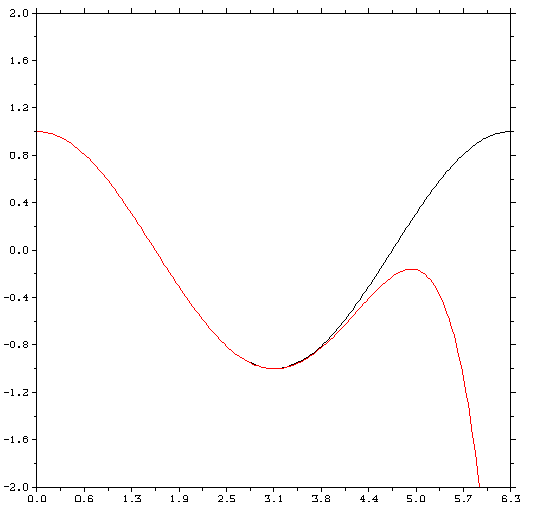
\includegraphics[width = \textwidth]{./doc/Figures/Taylor1.png}  \\
        \caption{Cosine (black) and Taylor expansion around $x_0 = 0$ with $N = 10$}
        \label{fig:Taylor1}
    \end{subfigure}
    \hspace{\fill}
    \begin{subfigure}[h]{0.4\textwidth}
        \centering
        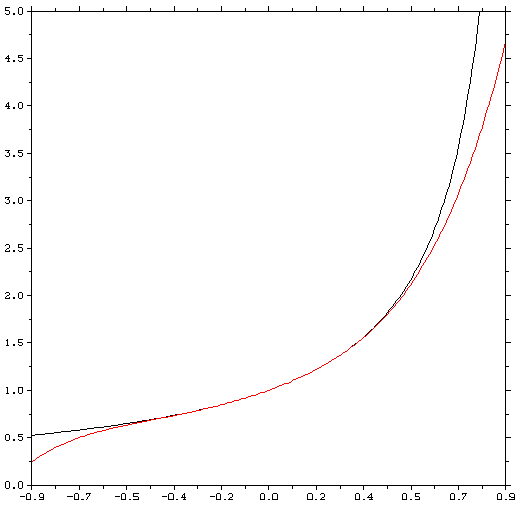
\includegraphics[width = \textwidth]{./doc/Figures/Taylor2.png}  \\
        \caption{Function $f(x) = \frac{1}{1-x}$ (black) and Taylor expansion around $x_0 = 0$ with $N = 5$}
        \label{fig:Taylor2}
    \end{subfigure}    

    \centering
    \begin{subfigure}[h]{0.4\textwidth}
        \centering
        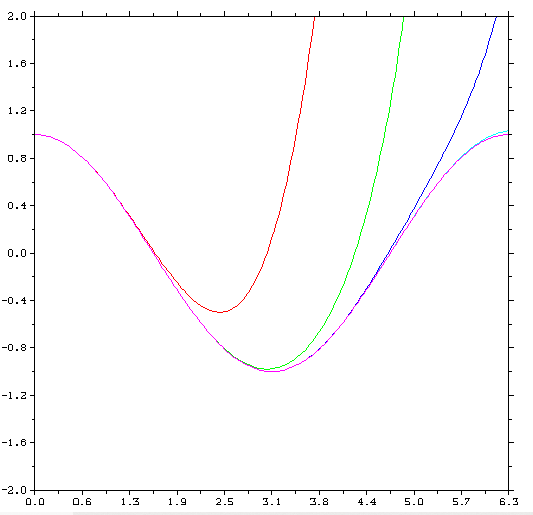
\includegraphics[width = \textwidth]{./doc/Figures/Taylor3.png}  \\
        \caption{Cosine (black) and different Taylor expansions around $x_0 = 0$ with $N = 1, 5, 9, 13, 17, 21$ and $25$}
        \label{fig:Taylor3}
    \end{subfigure}
    \caption{Different Taylor expansions for functions.}   \label{fig:Taylor}
\end{figure}


  
 
            \newpage 
            \subsubsection*{Python code} 
 The same functions are coded now with Python, notice that overloading both into one function called \texttt{Taylor} is performed in a 
 different way.
 
 \vspace{0.5cm}
 \renewcommand{\home}{./Python/sources/Foundations/Calculus} 
 \lstpython
 \listingsp{\home/Taylor_expansions.py}{def Taylor}
 {exit}{Taylor_expansions.py}
 
 
 \listingsp{\home/Taylor_expansions.py}{def Taylor_e}
 {Sigma}{Taylor_expansions.py}
  

 \listingsp{\home/Taylor_expansions.py}{def Taylor_N}
 {Sigma}{Taylor_expansions.py}
  
 
    
   
   \newpage 
   Try the same examples treated with Fortran in the Python project attached to this book:
      
   \vspace{0.5cm}
   \listingsp{\home/Examples/Series_expansion.py}{def Taylor_expansion_examples}
   {end}{Series_expansion.py}
   \lstfor
   
   
   
   
 % Taylor_expansion_examples
  
  
  
  
  
   
        %\newpage 
        %%___________________________________________________________________________________________________
        %\subsection{Parseval's identity} 
%
%Let's consider a function $f(x)$ and its Fourier series expansion, whether expressed as a sines-cosines expansion:
%\begin{equation} 
%	f ( x)  =  \sum_{k=0} ^{\infty} \  \hat{a}_k  \ \cos\left(k x\right)  + \sum_{k=1} ^{\infty} \  \hat{b}_k  \sin\left(k x\right)
%\end{equation} 	
%
%or as a complex form:
%\begin{equation} 
%    f ( x)  =  \sum_{k=-\infty} ^{\infty}  \hat{c}_k  e^{ i k x }
%\end{equation} 
%
%Notice that for this expressions the function $f(x)$ is considered real-valued and periodic with period $T=2\pi$. As we know, the computer 
%can not compute an infinite number of terms, we must truncate the series somewhere, let's say when $k = N-1$ so a total of $N$ terms are 
%considered. Then, the expansion becomes:
%\begin{equation} 
%    f ( x)  =  \sum_{k=0} ^{N-1} \  \hat{a}_k  \ \cos\left(k x\right) + \sum_{k=1} ^{N-1} \  \hat{b}_k  \sin \left(k x\right)
%\end{equation}
%
%or in complex form, those $N$ terms becomes:
%\begin{equation} 
%    f ( x)  =  \sum_{k=-\frac{N}{2}} ^{\frac{N}{2}-1}  \hat{c}_k  e^{ i k x }
%\end{equation} 
%
%We can quickly revise the relation between the coefficients of the sines-cosines expansion and the coefficients of the complex series 
%expansion:  
%
%$$
%\begin{cases}
%    \hat{c}_k  =  \frac{1}{2} \ ( \ \hat{a}_k  - i \ \hat{b}_k \ ),  \quad k=1, \ldots, N/2.   \\
%    \hat{c}_0  = \hat{a}_0   \\
%    \hat{c}_{-k}  =  \overline{ \hat{c} } _{k}  , \quad k=1, \ldots, N/2. 
%\end{cases}
%$$
%
%With that in mind, the Parseval's identity says:
%\begin{equation} 
%	\int _{-\pi} ^{\pi} f(x)^2 \ dx =  2 \pi  \sum_{k=-\infty} ^{\infty}  | \hat{c}_k | ^2       =  2 \pi \left(    | \hat{c}_0 |^2 + 2 
%	\sum_{k=1} ^{\infty} |  \hat{c}_k  |^2 \right) 
%\end{equation} 
%
%
%
%
%
%A good example, related to previous chapters, is the following: consider the function $ f(x) = x \quad $ $ \forall x \in [-\pi, +\pi ) $ and 
%extend it periodically to the right and to the left. Once $ f(x) $ is defined in this way, it can be approximated by a sine expansion: 
%%\begin{equation} 
%%	f ( x)  =  \sum_{k=1} ^{N/2} \   \hat{b}_k  \sin k x, 
%%\end{equation} 
%\begin{equation} 
%	f ( x )  =  \sum_{k=1} ^{\infty} \   \hat{b}_k  \sin \left(  kx\right), 
%\end{equation} 
%where the coefficients $ \hat{b}_k $ are given by:
%%\begin{equation} 
%%	\hat{b}_k   = \frac{ (-1)^{k+1} }{ \pi k }, \qquad k=1, \ldots, N/2. 
%%\end{equation} 
%\begin{equation} 
%    \hat{b}_k   = \frac{ 2 (-1)^{k+1} }{ k }, \qquad k=1, \ldots,\infty. 
%\end{equation} 
%
%Using the Parseval's identity with $f(x)$:
%$$
%\int_{-\pi}^{\pi}  x^2 dx  = \frac{2}{3} \pi^3 = 2\pi \left(   2\sum_{k=1}^{\infty}  \mid  -\frac{1}{2} i \hat{b}_k   \mid ^2  \right)
%$$
%
%and the following summation is obtained: 
%%\begin{equation} 
%%	\sum_{k=1} ^{\infty} \  \frac{1}{n^2}  \  = \frac{\pi^2}{6}
%%\end{equation} 
%\begin{equation} 
%    \sum_{k=1} ^{\infty} \  \frac{1}{k^2}  \  = \frac{\pi^2}{6}
%\end{equation}
%

        \newpage 
        \subsection{Truncated Fourier series}
Fourier series are important expansions in applied mathematics or physics to represent a
periodic functions.  
When implementing these expansions in the computer, truncated Fourier series are used
to approximate the infinity Fourier expansion.  
A truncated Fourier series is a finite sum of sine and cosine waves. 
$$
f(x) = \sum_{k=0}^N a_k \ \cos( \ 2 \pi k  x \ ) + b_k \ \sin ( \ 2 \pi k  x \ ), 
$$
or expressed in its compact form: 
$$
f(x) = \sum_{k=-N/2}^{N/2-1} c_k \ e^{ \ 2 \pi k  x \ i } .
$$
If $ f(x)$ is real, $ c_k $ and $a_k,\  b_k$ are related with the following expressions: 
$$
c_k = \frac{1}{2}(a_k - i b_k), \qquad k=0, \ldots, N/2, 
$$
$$
c_{-k} = \overline{c_k},\qquad k=1, \ldots, N/2,
$$
where $ k $ represents different harmonics of frequency or wavelength  $ 2 \pi k $  of different 
 sine and cosine components.

The following saw-tooth wave: 
$$
f(x) =
\left\{
\begin{array}{ll}
\displaystyle                          
\frac{x}{\pi}, \hspace{1cm} \hspace{2cm} &  \displaystyle  0 \leq x \leq  \pi,      \\ \\
\displaystyle                                                            
\frac{x}{\pi} -2 ,  & \displaystyle    \pi < x <  2 \pi. 
\\                                                                                                 
\end{array}                                                                   
\right.                                                     
$$
is expanded in Fourier series
$$
f(x) =\sum_{k=1}^N  - \frac{2 \ (-1)^{k}}{\pi \ k}   \ \sin ( \ 2 \pi k  x \ ).
\label{sawtooth}
$$



        \newpage
        \subsubsection*{Fortran}
In following Fortran code, the saw--tooth wave is reconstructed 
by means of its harmonic decomposition. The function \verb|Fourier_series| implements 
equation (\ref{sawtooth}). Then,  subroutine \verb|Fourier_example| calculates the image of 
\verb|M=2000| points to plot the resulting graph. 
\vspace{0.5cm} 
\renewcommand{\home}{./Fortran/sources/Advanced_programming/functional programming} 
\lstfor 
\listings{\home/Fourier.f90}
{elemental function Fourier_series}
{end function}{Fourier.f90}
\vspace{0.25cm}
\listings{\home/Fourier.f90}
 {subroutine Fourier_example}
 {end subroutine}{Fourier.f90}


        \newpage
        \subsubsection*{Python}
In following Python code, the saw--tooth wave is reconstructed 
by means of its harmonic decomposition. The function \verb|Fourier_series| implements 
equation (\ref{sawtooth}). Then, function \verb|Fourier_example| calculates the image of 
\verb|M=2000| points to plot the resulting graph. 
\vspace{0.5cm} 
\renewcommand{\home}{./Python/sources/Foundations/Algebra} 
\lstpython
 \listingsp{\home/Fourier.py}
 {def Fourier_example}
 {plt.show}{Fourier.py}


\listingsp{\home/Fourier.py}
{def Fourier_series}
{return}{Fourier.f90}

  
  
  